\documentclass[11pt,]{article}
\usepackage[]{mathpazo}
\usepackage{amssymb,amsmath}
\usepackage{ifxetex,ifluatex}
\usepackage{fixltx2e} % provides \textsubscript
\ifnum 0\ifxetex 1\fi\ifluatex 1\fi=0 % if pdftex
  \usepackage[T1]{fontenc}
  \usepackage[utf8]{inputenc}
\else % if luatex or xelatex
  \ifxetex
    \usepackage{mathspec}
  \else
    \usepackage{fontspec}
  \fi
  \defaultfontfeatures{Ligatures=TeX,Scale=MatchLowercase}
\fi
% use upquote if available, for straight quotes in verbatim environments
\IfFileExists{upquote.sty}{\usepackage{upquote}}{}
% use microtype if available
\IfFileExists{microtype.sty}{%
\usepackage{microtype}
\UseMicrotypeSet[protrusion]{basicmath} % disable protrusion for tt fonts
}{}
\usepackage[margin=1in]{geometry}
\usepackage{hyperref}
\hypersetup{unicode=true,
            pdftitle={Case Study Elections Netherlands},
            pdfauthor={Ilse van Beelen, Floor Komen and Lotte Pater},
            pdfkeywords={put some keywords here},
            pdfborder={0 0 0},
            breaklinks=true}
\urlstyle{same}  % don't use monospace font for urls
\usepackage{natbib}
\bibliographystyle{plainnat}
\usepackage{color}
\usepackage{fancyvrb}
\newcommand{\VerbBar}{|}
\newcommand{\VERB}{\Verb[commandchars=\\\{\}]}
\DefineVerbatimEnvironment{Highlighting}{Verbatim}{commandchars=\\\{\}}
% Add ',fontsize=\small' for more characters per line
\usepackage{framed}
\definecolor{shadecolor}{RGB}{248,248,248}
\newenvironment{Shaded}{\begin{snugshade}}{\end{snugshade}}
\newcommand{\KeywordTok}[1]{\textcolor[rgb]{0.13,0.29,0.53}{\textbf{#1}}}
\newcommand{\DataTypeTok}[1]{\textcolor[rgb]{0.13,0.29,0.53}{#1}}
\newcommand{\DecValTok}[1]{\textcolor[rgb]{0.00,0.00,0.81}{#1}}
\newcommand{\BaseNTok}[1]{\textcolor[rgb]{0.00,0.00,0.81}{#1}}
\newcommand{\FloatTok}[1]{\textcolor[rgb]{0.00,0.00,0.81}{#1}}
\newcommand{\ConstantTok}[1]{\textcolor[rgb]{0.00,0.00,0.00}{#1}}
\newcommand{\CharTok}[1]{\textcolor[rgb]{0.31,0.60,0.02}{#1}}
\newcommand{\SpecialCharTok}[1]{\textcolor[rgb]{0.00,0.00,0.00}{#1}}
\newcommand{\StringTok}[1]{\textcolor[rgb]{0.31,0.60,0.02}{#1}}
\newcommand{\VerbatimStringTok}[1]{\textcolor[rgb]{0.31,0.60,0.02}{#1}}
\newcommand{\SpecialStringTok}[1]{\textcolor[rgb]{0.31,0.60,0.02}{#1}}
\newcommand{\ImportTok}[1]{#1}
\newcommand{\CommentTok}[1]{\textcolor[rgb]{0.56,0.35,0.01}{\textit{#1}}}
\newcommand{\DocumentationTok}[1]{\textcolor[rgb]{0.56,0.35,0.01}{\textbf{\textit{#1}}}}
\newcommand{\AnnotationTok}[1]{\textcolor[rgb]{0.56,0.35,0.01}{\textbf{\textit{#1}}}}
\newcommand{\CommentVarTok}[1]{\textcolor[rgb]{0.56,0.35,0.01}{\textbf{\textit{#1}}}}
\newcommand{\OtherTok}[1]{\textcolor[rgb]{0.56,0.35,0.01}{#1}}
\newcommand{\FunctionTok}[1]{\textcolor[rgb]{0.00,0.00,0.00}{#1}}
\newcommand{\VariableTok}[1]{\textcolor[rgb]{0.00,0.00,0.00}{#1}}
\newcommand{\ControlFlowTok}[1]{\textcolor[rgb]{0.13,0.29,0.53}{\textbf{#1}}}
\newcommand{\OperatorTok}[1]{\textcolor[rgb]{0.81,0.36,0.00}{\textbf{#1}}}
\newcommand{\BuiltInTok}[1]{#1}
\newcommand{\ExtensionTok}[1]{#1}
\newcommand{\PreprocessorTok}[1]{\textcolor[rgb]{0.56,0.35,0.01}{\textit{#1}}}
\newcommand{\AttributeTok}[1]{\textcolor[rgb]{0.77,0.63,0.00}{#1}}
\newcommand{\RegionMarkerTok}[1]{#1}
\newcommand{\InformationTok}[1]{\textcolor[rgb]{0.56,0.35,0.01}{\textbf{\textit{#1}}}}
\newcommand{\WarningTok}[1]{\textcolor[rgb]{0.56,0.35,0.01}{\textbf{\textit{#1}}}}
\newcommand{\AlertTok}[1]{\textcolor[rgb]{0.94,0.16,0.16}{#1}}
\newcommand{\ErrorTok}[1]{\textcolor[rgb]{0.64,0.00,0.00}{\textbf{#1}}}
\newcommand{\NormalTok}[1]{#1}
\usepackage{graphicx,grffile}
\makeatletter
\def\maxwidth{\ifdim\Gin@nat@width>\linewidth\linewidth\else\Gin@nat@width\fi}
\def\maxheight{\ifdim\Gin@nat@height>\textheight\textheight\else\Gin@nat@height\fi}
\makeatother
% Scale images if necessary, so that they will not overflow the page
% margins by default, and it is still possible to overwrite the defaults
% using explicit options in \includegraphics[width, height, ...]{}
\setkeys{Gin}{width=\maxwidth,height=\maxheight,keepaspectratio}
\IfFileExists{parskip.sty}{%
\usepackage{parskip}
}{% else
\setlength{\parindent}{0pt}
\setlength{\parskip}{6pt plus 2pt minus 1pt}
}
\setlength{\emergencystretch}{3em}  % prevent overfull lines
\providecommand{\tightlist}{%
  \setlength{\itemsep}{0pt}\setlength{\parskip}{0pt}}
\setcounter{secnumdepth}{0}
% Redefines (sub)paragraphs to behave more like sections
\ifx\paragraph\undefined\else
\let\oldparagraph\paragraph
\renewcommand{\paragraph}[1]{\oldparagraph{#1}\mbox{}}
\fi
\ifx\subparagraph\undefined\else
\let\oldsubparagraph\subparagraph
\renewcommand{\subparagraph}[1]{\oldsubparagraph{#1}\mbox{}}
\fi

%%% Use protect on footnotes to avoid problems with footnotes in titles
\let\rmarkdownfootnote\footnote%
\def\footnote{\protect\rmarkdownfootnote}

%%% Change title format to be more compact
\usepackage{titling}

% Create subtitle command for use in maketitle
\newcommand{\subtitle}[1]{
  \posttitle{
    \begin{center}\large#1\end{center}
    }
}

\setlength{\droptitle}{-2em}

  \title{Case Study Elections Netherlands}
    \pretitle{\vspace{\droptitle}\centering\huge}
  \posttitle{\par}
    \author{Ilse van Beelen, Floor Komen and Lotte Pater}
    \preauthor{\centering\large\emph}
  \postauthor{\par}
      \predate{\centering\large\emph}
  \postdate{\par}
    \date{december 14, 2018}


\begin{document}
\maketitle
\begin{abstract}
Put the abstract over here
\end{abstract}

\section{1. Introduction}\label{introduction}

In this report the election

\subsection{1.1 Summary data}\label{summary-data}

In this chapter the data is summarized and explained how the data is
collected. The percentage of votes per party per municipality were found
on
\url{https://data.overheid.nl/data/dataset/verkiezingsuitslag-tweede-kamer-2017}.
The demographics; \emph{amount of non-west residents per municipality},
\emph{the urban index of a municipality} and \emph{the standardized
income per municipality}, were found on the CBS site. This is the Dutch
central office of statistics.

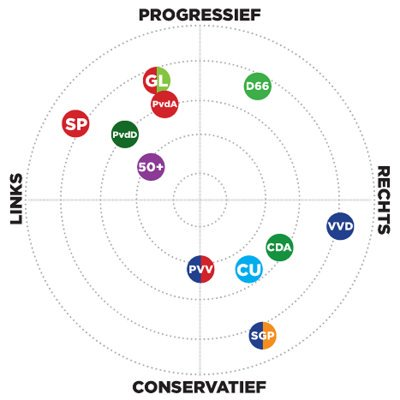
\includegraphics[width=2.60417in]{Partijlandschap.jpg} \textbf{Dutch
political parties}\\
In this landscape the diffence between the parties is graphically
displayed in this figure. In this research, two parties are chosen to
investigate. These two parties had to be different, so that some
comparisons could be made. The parties should not be to extreme
left/right/conservative/progressive, so that the model will be proven to
work on less-extreme parties. Therefore, the chosen parties are: CDA and
GroenLinks. After the data-cleaning the CDA will be researched first,
afterwards GroenLinks will be researched.

\textbf{Demographics}\\
In this research the above described demographics are chosen because of
there influence on a municipality level. The thought is that a more
non-western municipality for example votes different than a less
non-western municipality. This is the same for the other two
demographics. Other demographics are also researched, for example
gender, but on a municipality level there is no big difference between
the amount of men and women per municipality. So that is a more
interesting demographic to research on an individual level. \emph{The
standardized income per municipality} are given in thousands. \emph{the
urban index of a municipality} is a database with five categories per
municipality. These five categories are; really strong urban (more than
2500 addresses per km2), strong urban (1500-2500 addresses per km2),
moderate urban (1000- 1500 addresses per km2), little urban (500-1000
addresses per km2) and not urban (less than 500 addresses per km2). Per
municipality the amount of km2 per category is given. The \emph{non-west
residents per municipality} is given in an amount per municipality, also
the total amount of residents is given per municipality.

\subsection{1.2 Data cleaning}\label{data-cleaning}

The variable \emph{non-western residents} are divided in three groups.
Municipalities with less than 5 \% non-western residents, 5-10 \%
non-western residents and municipalities with more dan 10 \% non-western
residents.

\begin{Shaded}
\begin{Highlighting}[]
\KeywordTok{setwd}\NormalTok{(}\StringTok{"~/Studie/Statistics & Data Science/Semester 1/Lineair models and Algebra/CaseStudyLineair2018"}\NormalTok{)}
\NormalTok{Data <-}\StringTok{ }\KeywordTok{read.csv}\NormalTok{(}\StringTok{"1_clean_data/voting_and_demographics.csv"}\NormalTok{, }\DataTypeTok{stringsAsFactors =}\NormalTok{ F, }
    \DataTypeTok{header =}\NormalTok{ T)}
\NormalTok{Data <-}\StringTok{ }\NormalTok{Data[, }\OperatorTok{-}\DecValTok{15}\NormalTok{]}
\KeywordTok{colnames}\NormalTok{(Data) <-}\StringTok{ }\KeywordTok{c}\NormalTok{(}\StringTok{"Muni"}\NormalTok{, }\StringTok{"VVD"}\NormalTok{, }\StringTok{"CDA"}\NormalTok{, }\StringTok{"PVV"}\NormalTok{, }\StringTok{"D66"}\NormalTok{, }\StringTok{"SP"}\NormalTok{, }\StringTok{"GL"}\NormalTok{, }\StringTok{"PvdA"}\NormalTok{, }
    \StringTok{"CU"}\NormalTok{, }\StringTok{"50PLUS"}\NormalTok{, }\StringTok{"PvdD"}\NormalTok{, }\StringTok{"SGP"}\NormalTok{, }\StringTok{"FvD"}\NormalTok{, }\StringTok{"DENK"}\NormalTok{, }\StringTok{"Urban_index"}\NormalTok{, }\StringTok{"High_edu_perc"}\NormalTok{, }
    \StringTok{"Mean_income"}\NormalTok{, }\StringTok{"Dutch_perc"}\NormalTok{, }\StringTok{"West_perc"}\NormalTok{, }\StringTok{"Non_west_perc"}\NormalTok{)}
\NormalTok{Data}\OperatorTok{$}\NormalTok{Non_west <-}\StringTok{ }\KeywordTok{ifelse}\NormalTok{(Data}\OperatorTok{$}\NormalTok{Non_west_perc }\OperatorTok{<}\StringTok{ }\FloatTok{0.05}\NormalTok{, }\DecValTok{1}\NormalTok{, }\OtherTok{NA}\NormalTok{)}
\NormalTok{Data}\OperatorTok{$}\NormalTok{Non_west <-}\StringTok{ }\KeywordTok{ifelse}\NormalTok{(Data}\OperatorTok{$}\NormalTok{Non_west_perc }\OperatorTok{>=}\StringTok{ }\FloatTok{0.05} \OperatorTok{&}\StringTok{ }\NormalTok{Data}\OperatorTok{$}\NormalTok{Non_west_perc }\OperatorTok{<}\StringTok{ }\FloatTok{0.1}\NormalTok{, }
    \DecValTok{2}\NormalTok{, Data}\OperatorTok{$}\NormalTok{Non_west)}
\NormalTok{Data}\OperatorTok{$}\NormalTok{Non_west <-}\StringTok{ }\KeywordTok{ifelse}\NormalTok{(Data}\OperatorTok{$}\NormalTok{Non_west_perc }\OperatorTok{>=}\StringTok{ }\FloatTok{0.1}\NormalTok{, }\DecValTok{3}\NormalTok{, Data}\OperatorTok{$}\NormalTok{Non_west)}
\NormalTok{Data}\OperatorTok{$}\NormalTok{Non_west <-}\StringTok{ }\KeywordTok{as.factor}\NormalTok{(Data}\OperatorTok{$}\NormalTok{Non_west)}
\NormalTok{Dat_cda <-}\StringTok{ }\NormalTok{Data[, }\KeywordTok{c}\NormalTok{(}\DecValTok{1}\NormalTok{, }\DecValTok{3}\NormalTok{, }\DecValTok{15}\NormalTok{, }\DecValTok{16}\NormalTok{, }\DecValTok{17}\NormalTok{, }\DecValTok{21}\NormalTok{)]}
\NormalTok{Dat_cda <-}\StringTok{ }\NormalTok{Dat_cda[}\KeywordTok{complete.cases}\NormalTok{(Dat_cda), ]}
\end{Highlighting}
\end{Shaded}

\subsection{1.3 Data visualisation}\label{data-visualisation}

\subsubsection{CDA}\label{cda}

In this part the cleaned data is visualized, so that a good picture can
be obtained of the current data. First of all some demographics of data
will be showed. In these histograms the density of the \emph{CDA},
\emph{the urban index}, \emph{the percentage of highly educated
residents} and \emph{the mean income} are plotted.

\begin{center}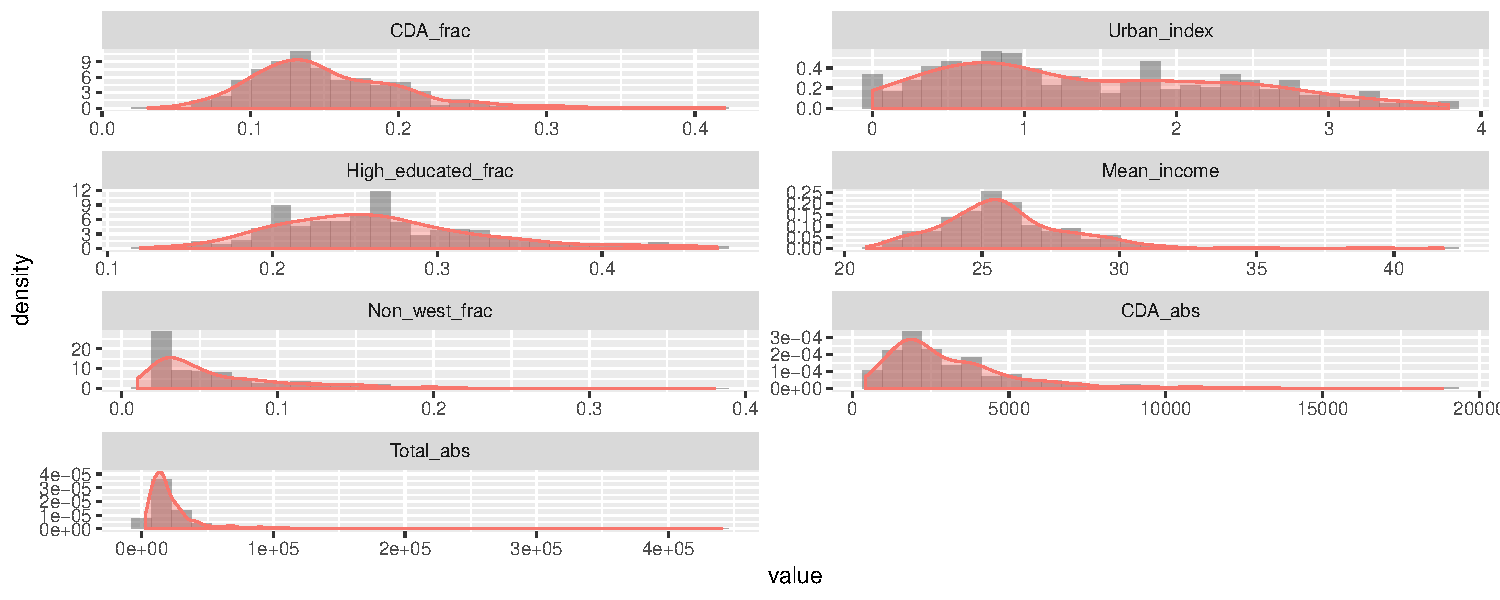
\includegraphics{Report_files/figure-latex/demographics_data-1} \end{center}

\textbf{Correlation heatmap} In this heatmap the correlation between
explanatory and respons variable are showed. The red color means a
positive relation, the purple color means a negative relation. The
relation between \emph{mean income} and \emph{percentage highly
educated} is the highest.

\begin{center}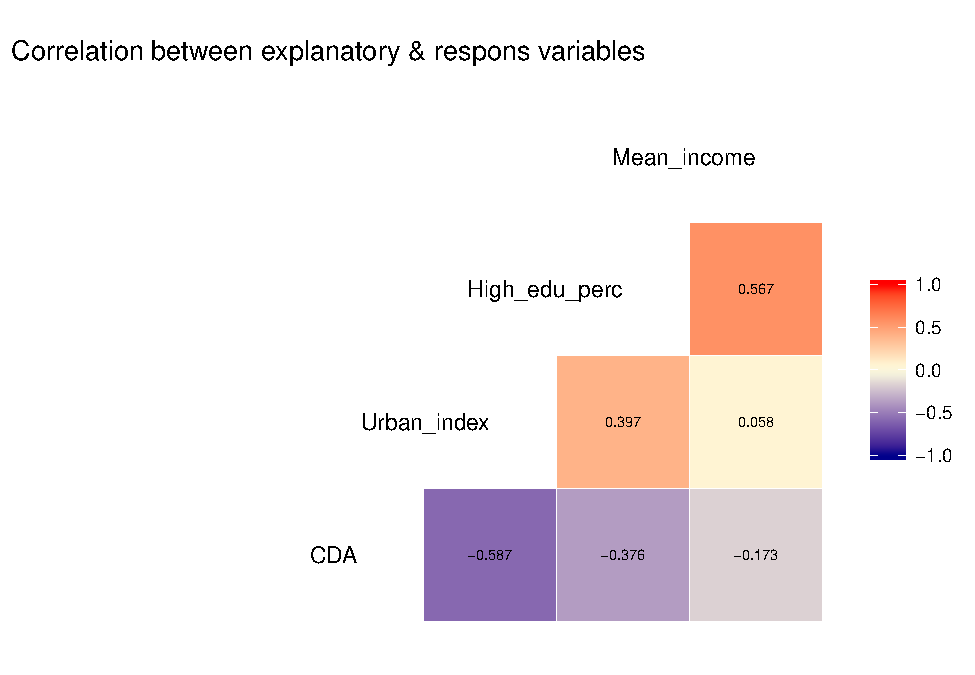
\includegraphics{Report_files/figure-latex/correlation_heatmap-1} \end{center}

\begin{verbatim}
## [1] 0.02985029
\end{verbatim}

\textbf{multiplot}

\begin{center}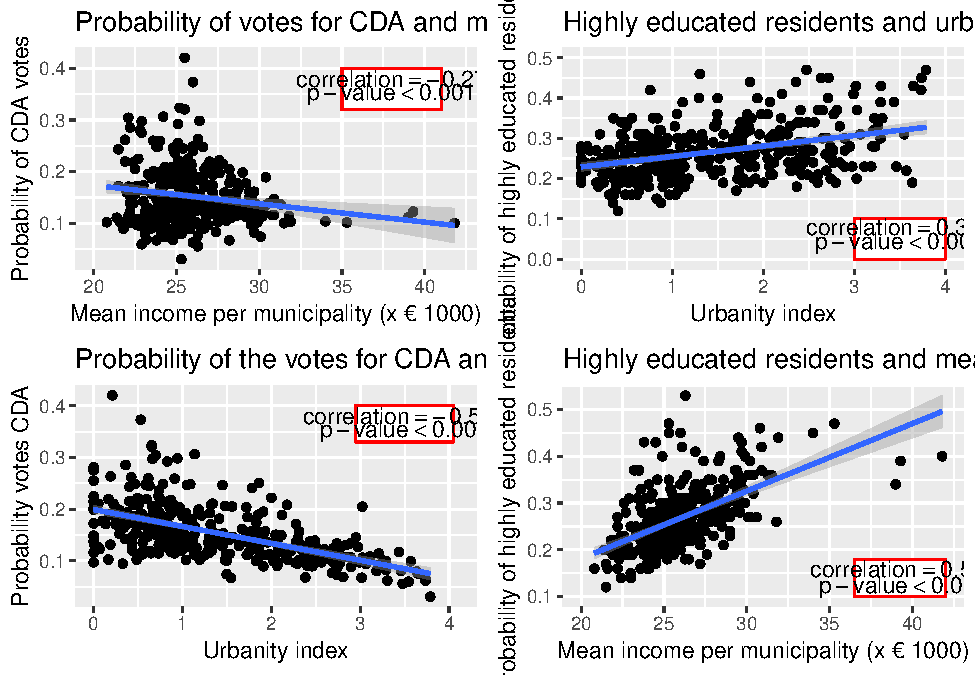
\includegraphics{Report_files/figure-latex/multi_plots-1} \end{center}

\textbf{boxplots}

\begin{center}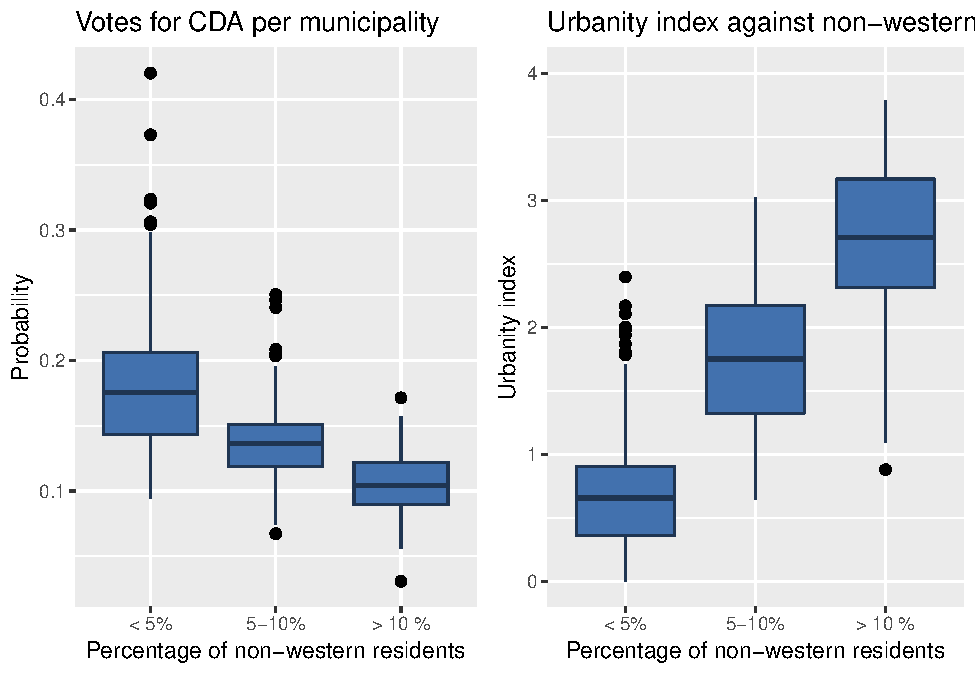
\includegraphics{Report_files/figure-latex/multi_boxplots-1} \end{center}

\subsubsection{Groenlinks}\label{groenlinks}

\section{2. Formulate model}\label{formulate-model}

Model formuleren

\subsection{CDA}\label{cda-1}

\subsection{GroenLinks}\label{groenlinks-1}

\section{3 Final model}\label{final-model}

\subsection{CDA}\label{cda-2}

\subsection{Groenlinks}\label{groenlinks-2}

\section{4 Analyse output}\label{analyse-output}

\section{5 Discussion}\label{discussion}

\subsection{5.1 Limitations}\label{limitations}


\end{document}
